\documentclass[11pt]{article}

%%% Load some useful packages:
%% "New" LaTeX2e graphics support.
\usepackage{graphicx}
%%	using final option to force graphics to be included even in draft mode
%\usepackage[final]{graphicx}

%% Support sub-figures.
\usepackage{subfigure}

%% Make subsubsections numbered and included in ToC
\setcounter{secnumdepth}{3}
\setcounter{tocdepth}{3}

%% Package to linebreak URLs in a sane manner.
\usepackage{url}

%% Define a new 'smallurl' style for the package that will use a smaller font.
\makeatletter
\def\url@smallurlstyle{%
  \@ifundefined{selectfont}{\def\UrlFont{\sf}}{\def\UrlFont{\small\ttfamily}}}
\makeatother
%% Now actually use the newly defined style.
\urlstyle{smallurl}

%% Make margins less ridiculous
\usepackage{fullpage}

%% Allows insertion of fixme notes for future work
\usepackage[footnote, nomargin]{fixme}

%%%% Turned off for tech report, should be turned on for research portfolio
%% Turn on double spacing
%\usepackage{setspace}
%\doublespacing

%% Make URLs clickable
\usepackage[colorlinks, bookmarks=true]{hyperref}
\usepackage[all]{hypcap}


%% Since I'm using the LaTeX Makefile that uses dvips, I need this
%% package to make URLs break nicely
\usepackage{breakurl}

\usepackage{array}

%% Make table cross pages.
\usepackage{longtable}

\begin{document}

\title{Makahiki: A framework for serious games for sustainability\\
\em  A Research White Paper}

\author{
	 Yongwen Xu \\
\em  Collaborative Software Development Laboratory \\
\em  Department of Information and Computer Sciences \\
\em  University of Hawai'i at Manoa\\
     yxu@hawaii.edu \\
}

\date{\today}
\maketitle

\tableofcontents

\graphicspath{{figures/}} 
\DeclareGraphicsExtensions{.eps} 

\newpage
\begin{abstract}

My research seeks to investigate how to build a customizable serious game engine for sustainability called Makahiki. It provides an open source, component-based, extensible framework for creating serious games for the purpose of education and behavioral change regarding energy, water, food, and waste generation and use. Different organizations configures the Makahiki framework to produce a ``challange instance'' with a specific set of game mechanics, user interface features, and experimental goals. Makahiki provides sophisticated instrumentation to support evaluation of how well the game mechanics supported the organization's goals for the challenge.

This white paper describes the Makahiki's research goal, system design, and experimental design on how to evaluate the effectiveness of the Makahiki as framework in developing serious games for sustainability.
\end{abstract}


%% Contains introduction to the related work when used outside the
%% context of the dissertation proposal
\section{Introduction}

Sustainability education and conservation has become an international imperative due to the rising cost of energy, increasing scarcity of natural resources and irresponsible environmental practices. 
Over the past decade, running energy and water challenges have become a focal point for sustainability efforts at university, government, and industry campuses. Designers of those competitions have had three choices for information technology: (a) build their own custom in-house solution; (b) out-source to a commercial provider; or (c) use a "minimal tech" solution such as a web page and manual posting of data and results.

We developed a framework called Makahiki as a new choice: an extensible game engine for the development and evaluation of sustainability challenges. Makahiki has a unique feature set intended to foster more rapid innovation and development. These features include: (1) an open source license and development model which makes the technology available without charge and facilitates collaborative development and improvement; (2) support for an "ecosystem" of extensible, interrelated, customizable games and activities; (3) real-time game analytics and A/B testing for research and evaluation; (4) pedagogically organized and extensible learning activities; (5) a responsive user interface supporting mobile, tablet, and laptop displays; and (6) support for deployment to the cloud as an inexpensive option for hosting the competition.

The Makahiki framework will be used in 2012 by three organizations, namely, University of Hawaii at Manoa, Hawaii Pacific University, East West Center of University of Hawaii, to implement individually tailored sustainability challenges focusing on energy and water conservation. 

\section{Research Goals}

Makahiki intends to create synergy between the need to create knowledge and engagement regarding energy and the ability of so-called ``serious game'' techniques and energy feedback to create participation and engagement. In Makahiki, online game mechanics are employed with the goal of affecting real-world energy behaviors.  The ultimate goal is to not just affect energy behaviors during the course of the game, but to produce long lasting, sustained change in energy behaviors and outlooks by participants.

There are two research goals in Makahiki: (a) provides an extensible framework to easily create engaging games for sustainability education and behavior change, and (b) provides an experimental test bed for Gamification research into the effectiveness of different game mechanics in the context of sustainability.

The challenges of creating a customizable game engine are:  (a) creating a new instance of Makahiki by selecting the games they want the system to support, and (b) extending Makahiki by writing new game components, and (c) supporting ease of use by non-technical organizations with minimal technical support.

In order to provide an experimental test bed for game research, Makahiki will be designed to support A-B testing, where different game mechanics could be configured using the game engine to create ``treatments'' for different user groups. The game engine will provide real-time game analytics to these treatments.

\section{System Design}

Makahiki consists of a configurable game engine that can be customized to the needs of different organizations.  It includes a library of pre-built game ``widgets'' that implement a variety of game mechanics.  Using the widgets, an organization can create a custom energy challenge in which players can compete individually and/or in teams to earn the most points by reducing their energy consumption as well as by learning about energy concepts in general. Figure \ref{fig:makahiki-architecture} illustrates the architecture of Makahiki.

\begin{figure}[ht!]
  \center
  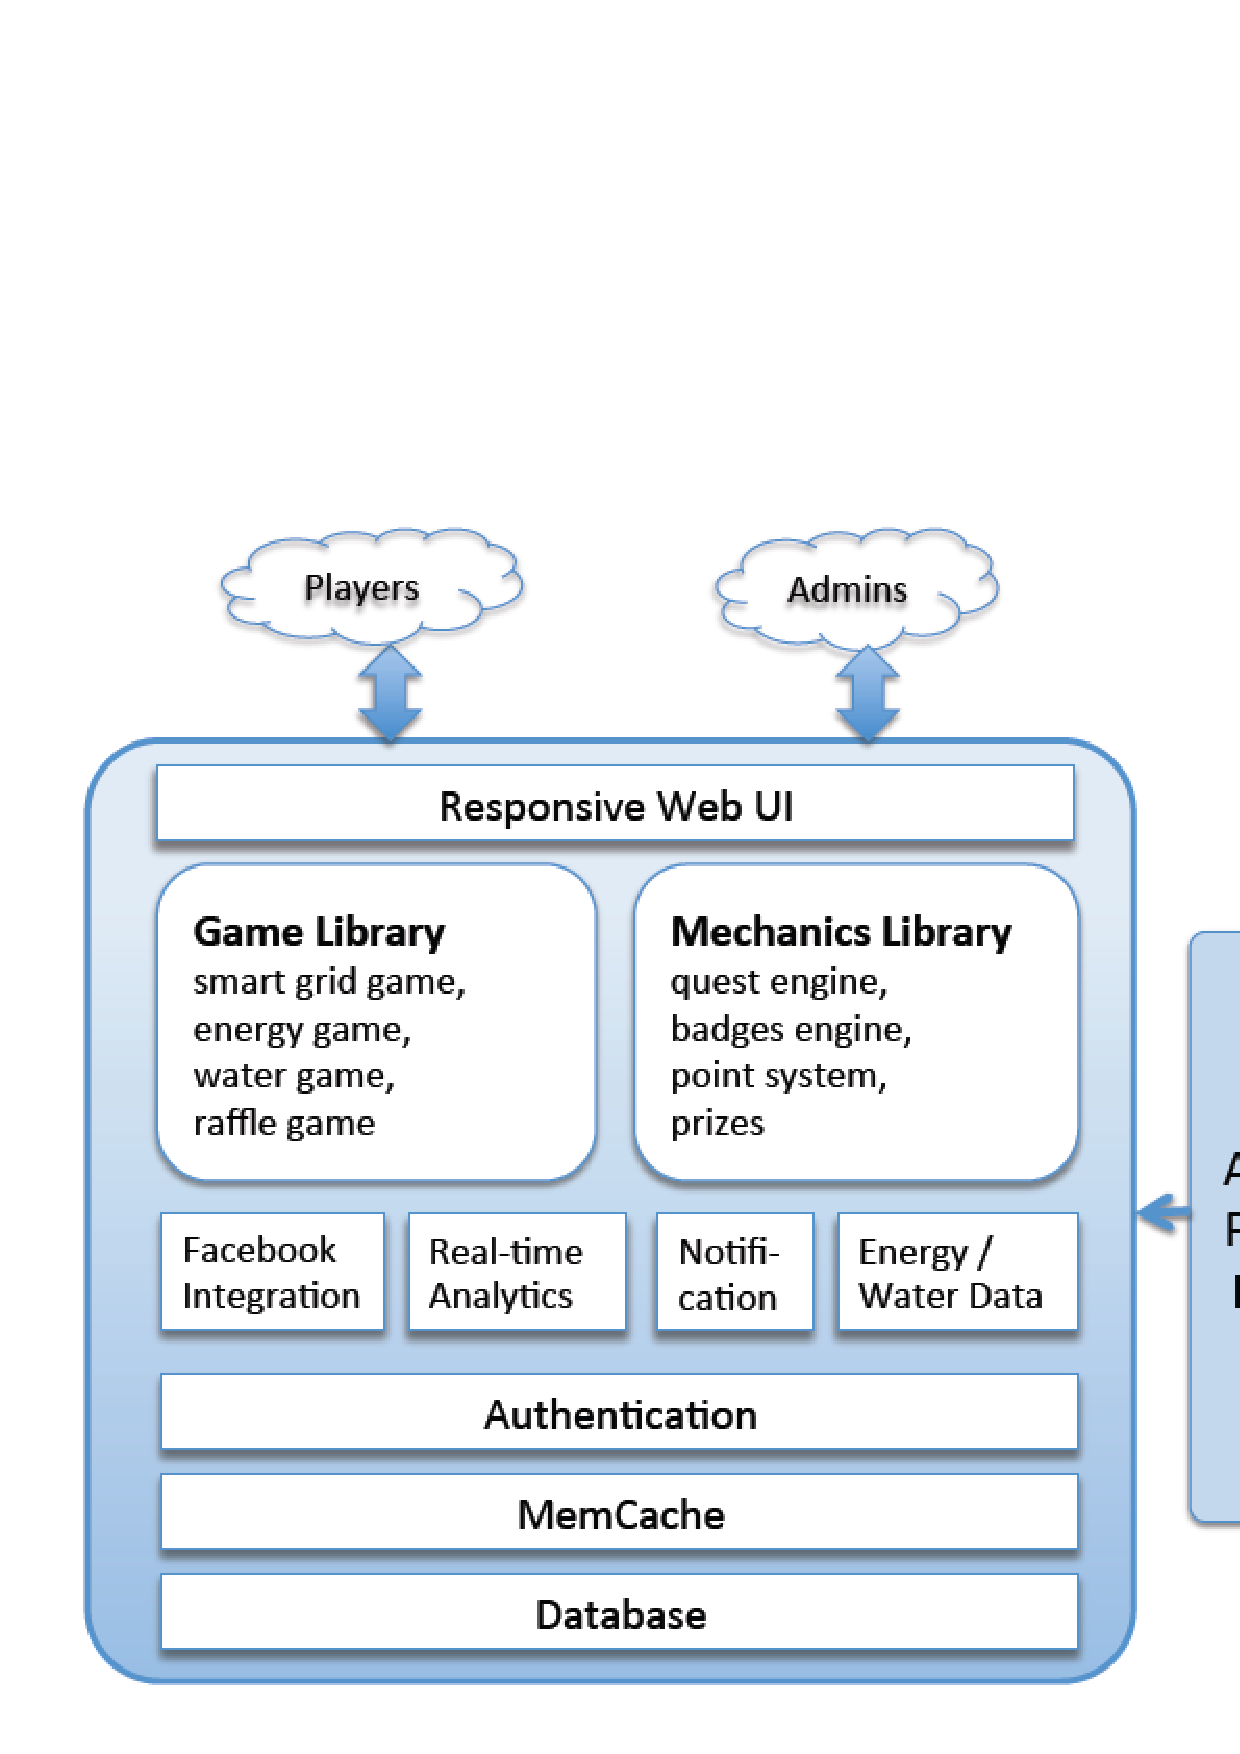
\includegraphics[width=0.6\textwidth]{makahiki-system-architecture}
  \caption{Architecture of Makahiki}
  \label{fig:makahiki-architecture}
\end{figure}

\begin{figure}[ht!]
	\centering
		\subfigure[Smart Grid Game]{\label{fig:SmartGrid}\includegraphics[height=2in]{smart-grid-game.eps}}
		\subfigure[Daily Energy Goal Game]{\label{fig:DailyEnergyGoal}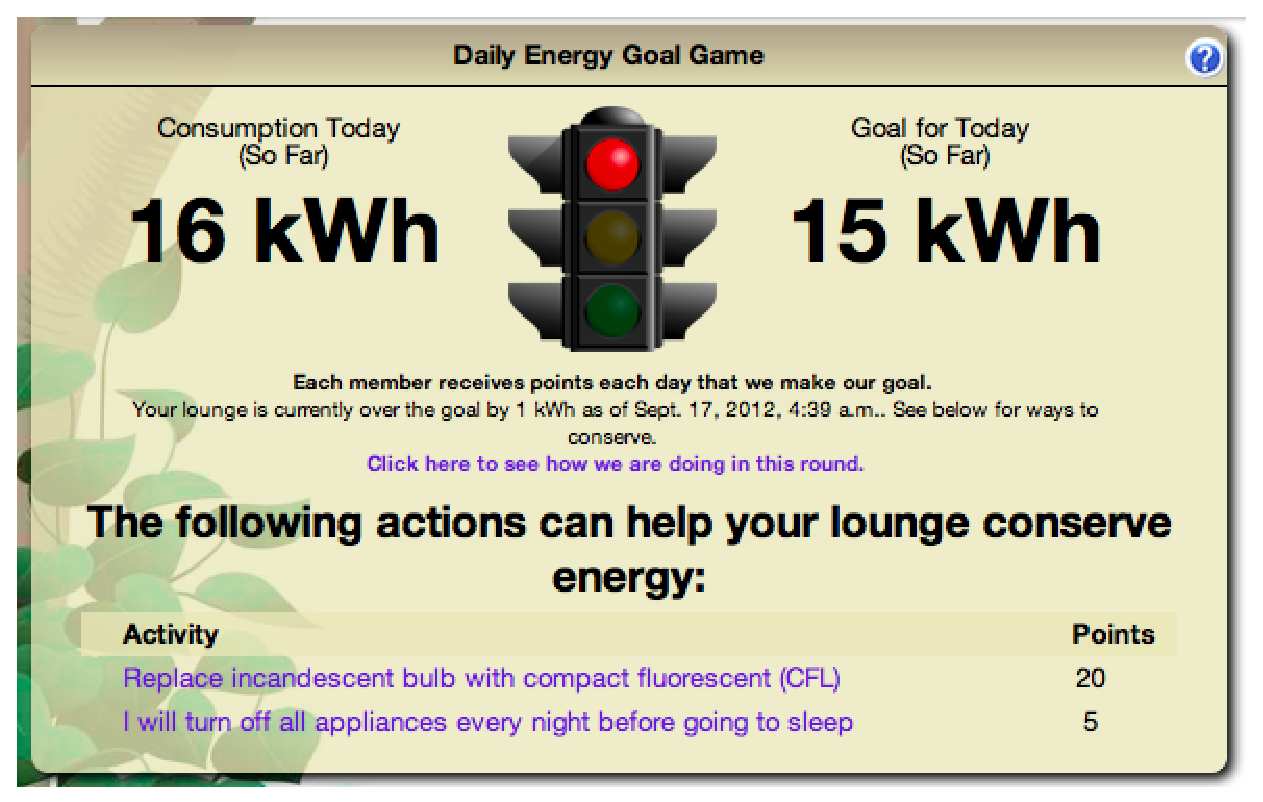
\includegraphics[height=2in]{daily-energy-goal-game.eps}}
		\subfigure[Raffle Game]{\label{fig:RaffleGame}\includegraphics[height=2in]{raffle-game.eps}}
		\caption{Makahiki Game Library}
		\label{fig:games}
\end{figure}

\subsubsection{Smart Grid Game}

The {\em Smart Grid Game widget}, shown in Figure \ref{fig:SmartGrid}, is the primary place players go to learn about energy issues and earn points. Actions are organized into a grid of squares (hence the name ``Smart Grid'') and organized by category columns. The grid contains four different types of actions: activities, commitments, events, and excursions. {\em Activities} are the most basic task available in the Smart Grid. In order to get points for an activity, a player will have to provide a response to the administrators. These responses can be a short textual answer or an uploaded picture. Administrators access a special admin section of the web application to approve or deny submissions. If a submission is approved, the player will receive the points for their submission. {\em Commitments} are pledges that the player will do something sustainable for a period of five days. {\em Events and excursions} are tied to real world activities that are held on or off campus. At the event, an administrator will hand out attendance codes printed on slips of paper that can be entered on the website by the players to earn points.

Not all of the tasks in the Smart Grid Game are necessarily available at the start of the game. We implemented a set of predicates that can be used to determine if a task is locked or unlocked for a player. For example, some activities will unlock when a certain number of tasks has been completed, or a certain date has been passed.

\subsubsection{Daily Energy Goal Game}

The {\em Daily Energy Goal Game widget}, shown in Figure \ref{fig:DailyEnergyGoal}, provides an actionable feedback to link between the energy conservation competition and the point competition. From this widget, Players can view their team's current energy consumption progress toward their daily energy goal, which is calculated from based on a baseline of the consumption of the previous 2 weeks. If the team did reach their goal at the end of the day, each member of the team that is participating in the game receives a configurable energy goal points.

\subsubsection{Raffle Game}

The {\em Raffle Game widget}, shown in Figure \ref{fig:RaffleGame}, provides a way to incentivize participation from all individuals, even those who are not in the running for a top prize. For every 25 points a player earns, they receive one virtual raffle ticket. Players can dynamically allocate their tickets to any raffle prizes they are interested in at any time, up to the end of the raffle.

\subsubsection{Real Time Game Analytics}

Makahiki also includes real-time game analytics that provides quantitative instrumentation to track when, where, and for how long each player accessed each page of the site and the interaction with each game components.  Unlike generic web server logs, this feature could track per-player game-specific behaviors in real-time. Figure \ref{fig:status} shows 2 examples of the game analytics components.

\begin{figure}[ht!]
	\centering
		\subfigure[User Stats]{\label{fig:user-stats}\includegraphics[width=0.45\textwidth]{user-stats.eps}}
		\subfigure[Energy Goal Game Stats]{\label{fig:goal-stats}\includegraphics[width=0.45\textwidth]{goal-stats.eps}}
		\caption{Real time game analytics}
		\label{fig:status}
\end{figure}

\section{Experimental Design}

In order to evaluate how the Makahiki meets the research goals, we propose to investigate the following the research questions:

\begin{enumerate}

\em \item Can Makahiki be successfully deployed in multiple organizational scenarios to provide games for major sustainability issues (energy, water, etc.)? \em
\em \item Can Makahiki provide an API and procedures to support enhancement with new features and capabilities with a minimum of impact on other aspects of the framework? \em
\em \item Can Makahiki provide an engaging and fun learning user interface to its end users? \em
\em \item Can Makahiki provide a mean to perform research on games for sustainability through real-time analytics and A/B testing? \em

\end{enumerate}

\subsection{Site Administration Case Study}
To evaluate question (1), we plan to perform the Site Administration Case Study research on multiple cases. It consists of structured interview process with the site administrators and the correlated data analysis of the archived email changes regarding the administration of the challenges.

\subsubsection{Methodology}

We plan to perform structured interviews to the site administrators of the Hawaii Pacific University (HPU) and East-West Center at Hawaii (EWC) Challenges. There are two site administrators for each site: one whose main role is responsible for the system installation, deployment of the application, etc; another whose main role is responsible for the challenge administration, including setting up the users, game settings, prizes, etc. The two sites have different deployment strategies: HPU will deploy the Makahiki instance in its own infrastructure, while EWC will deploy the instance into the Heroku Platform as a Service (PaaS) environment. The two case studies will provide insight into the differences of site administrations between a traditional self-hosting environment and an cloud based PaaS hosting environment.

We will undertake three interviews for each site administrator:
a. Pre-challenge interviews
b. In-challenge interviews
c. Post-challenge interviews
The Pre-challenge interviews happen before the challenge. They evaluate how easy or difficult for a system administrator and challenge administrator to install, setup, configure a challenge tailored to their specific requirements. The In-challenge interviews happen during the challenge. They evaluate the required work for administrating the site during the challenge. The Post-challenge interviews happen after the challenge. They evaluate the overall experience of the site administration.

We will record the structured interviews and archive the email exchanges with the site administrators for correlated data analysis.

\subsubsection{Data Analysis}
We will analyze both the quantitative and qualitative data collected from the interviews and email changes. The quantitative data include:
\begin{itemize}
 \item time taken to install the Makahiki
 \item time taken to configure the Challenge
 \item number of problems encountered
 \item time taken in training
 \item time taken in administrating the challenge
 \item number of problems encountered during the administrating of the challenge
 \item cost of the self-hosting v.s. cloud-based infrastructure
\end{itemize}

The qualitative data include:
\begin{itemize}
 \item What are the experiences of designing the game?
 \item What are the unique challenges for running their versions of Makahiki?
 \item What are the strenth of the administrative interface?
 \item What are the weekness of the administrative interface?
 \item How can we improve the administrative experience?
\end{itemize}

\subsection{Development Enhancement Case Study}
To evaluate question (2), we plan to perform the Development Enhancement Case Study research. It consists of one or several ``case study'' of external developers who are tasked with making an enhancement to the system.  The goal for the developer evaluation is to find out: (a) What kinds of learnings must occur, (b) What kind of background is necessary from a developer to enhance the system, (c) What kinds of problems were encountered and how they were resolved, (d) What kinds of changes to the system could be made to address the problems.

We plan to collect and analyze the data from the followings:
\begin{enumerate}
\item \em Log Book\em: We will create a google Form for the developer to fill out at the end of each programming session. Figure \ref{fig:developer-eval-form} illustrates the google form used for Makahiki developer evaluation.

\begin{figure}[ht!]
   \centering
   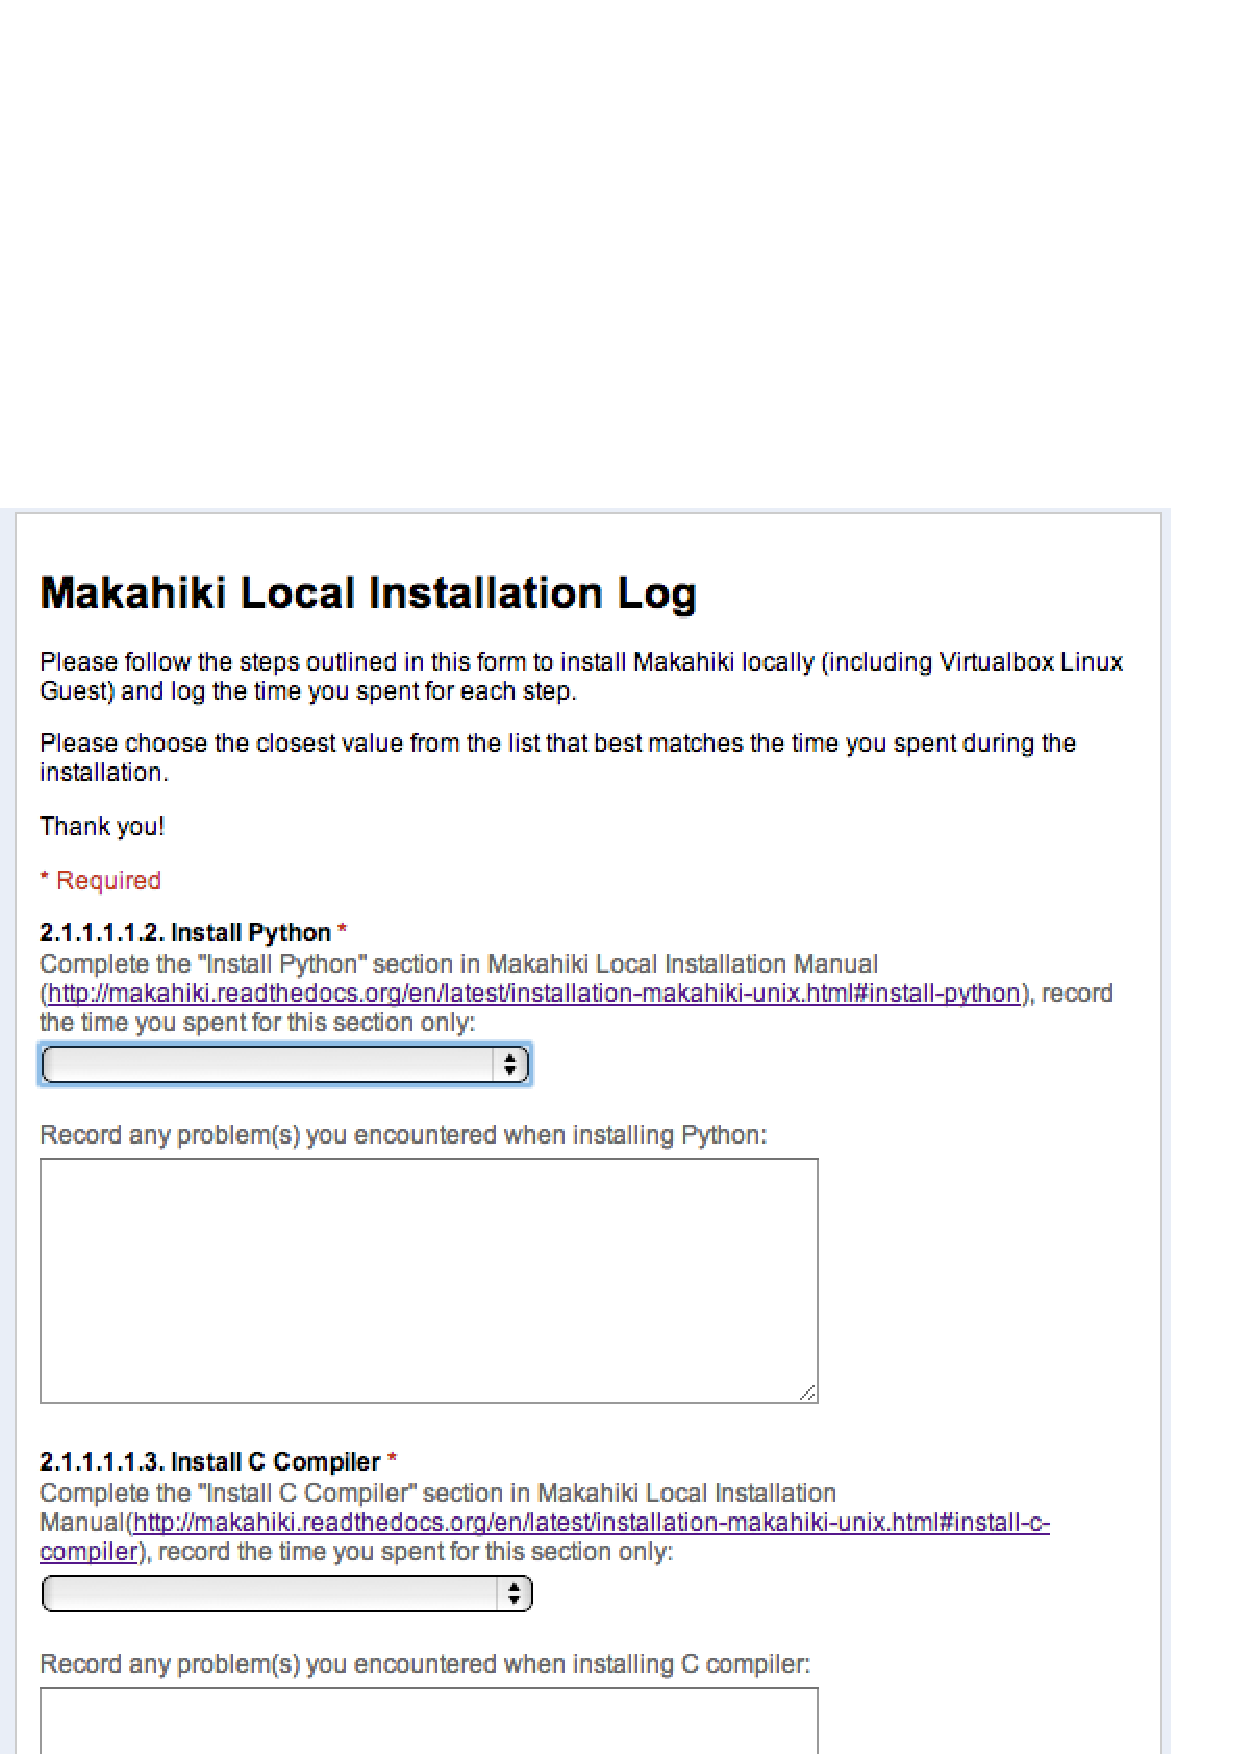
\includegraphics[height=30em,width=30em]{developer-eval-form}
   \caption{Makahiki Developer Evaluation Form}
   \label{fig:developer-eval-form}
\end{figure}
 
\item \em Meetings \em: We will have weekly developer meetings. we will record the meetings to support the analysis of development usability. we will focus on what kind of problems were encountered during the development.

\item \em Emails and Chat sessions \em: We will save the email exchanges with the developer and the online chat sessions for further analysis.

\item \em Code Review \em: We will review the development source code and documentation to identify the effectiveness of the enhancement and the impact to the whole application.

\end{enumerate}

\subsection{End User Evaluation}
To evaluate question (3), we plan to perform End User Evaluation with in-game survey and aggregated analytics from the logging data collected from all sites.

The \em in-game survey \em will be implemented as an activity action in smartgrid game in the challenge. Players can earn points by completing the survey action. We will use SurveyGizimo to create the survey which consists of a series of questions about the players' experiences with the game application. The response from the in-game survey will be analyzed via coding to provide insights about the end user expperiences of the Makahiki application.

We also plan to collect the logging data from all three sites to assess users' interaction with the system, as well as assessing the reliability and performance of the system.

The logging data will be analyzed to gather the following quantitative metrics:
\begin{itemize}
 \item Popular Quests, Events, Activities, Commitments, RSVPs
 \item Referrals
 \item Daily logins, New Users
 \item Action Feedbacks
 \item Errors occurred
 \item Numbers of long latency responses
\end{itemize}

\subsection{A/B Testing Evaluation Case Study}
To evaluate question (4), we plan to perform the case study research on at least one case. It consists of a ``case study" of one A/B test from three sites in order to answer the following research question: What level of energy data "latency" is required to provide useful feedback to participants in energy challenges like the Kukui Cup?  To assess this, we will implement three levels of energy latency:  (a) Subminute-level latency through the Power Meter at Hawaii Pacific University site; (b) Hour-level latency through the Daily Energy Goal Game at University of Hawaii site (no Power Meter); and (c) Day-level latency through the manual Daily Energy Goal Game at East West Center site.  In-game surveys will  be used at each site to determine how much participants interacted with the given type of feedback, and whether they felt limited by the given level of latency.

\section{Preliminary Results}
We designed and implemented an energy challenge called the ``Ku\-kui Cup'' for over 1,000 first year students living in the residence halls at the University of Hawaii in Fall, 2011. Response to this initial challenge was very positive. Over 400 students participated, for an adoption rate of approximately 40\%.  In the in-game survey of those participating students, over 90\% of them said they would play the game if it were offered next year.  60\% of participants said ``ease of use'' was the thing they liked best about the website.  40\% responded ``Nothing'' when asked what was confusing about the website, and 32\% responded ``Nothing'' when asked what they would change about the website.

 The 2012 Kukui Cup is currently being held in the residence halls at the University of Hawaii, and additional Kukui Cup challenges are happening at Hawaii Pacific University and the East-West Center. We are in the process of collecting the data both from the challenge administrators and from the student players.

\section{Selected publications}

[1] Beyond kWh: Myths and fixes for energy competition game design, In Proceedings of Meaningful Play 2012, Philip Johnson, Yongwen Xu, Robert Brewer, George Lee, Michelle Katchuck, Carleton Moore

[2] Makahiki+WattDepot: An open source software stack for next generation energy research and education, To appear in Proceedings of the 2012 Conference on Information and Communication Technologies for Sustainability (ICT4S), Philip M. Johnson, Yongwen Xu, Robert S. Brewer, George E. Lee, Andrea Connel

[3] Lights Off. Game On. The Kukui Cup: A Dorm Energy Competition,  In Proceedings of the CHI 2011 Workshop on Gamification (May 2011), Robert S. Brewer, George E. Lee, Yongwen Xu, Caterina Desiato, Michelle Katchuck, Philip M. Johnson

%% Use this for an alphabetically organized bibliography
%%\bibliography{sustainability,csdl-trs,gamification}
%%\bibliographystyle{plain}

\end{document}
